% @Author: Ren Qingjie
% @Date:   2017-06-06 13:58:21
% @Last Modified by:   Ren Qingjie
% @Last Modified time: 2017-06-11 08:54:45

\documentclass[10pt]{article}
\usepackage{threeparttable}
\usepackage{apacite}
\usepackage{graphicx}
\usepackage{multicol}
\usepackage{multirow}
\usepackage{caption}
\usepackage{extarrows}%为了输出长等号
\usepackage{subcaption}%为了插图
\usepackage[UTF8]{ctex}

\author{Jack}
\title{Time Series Analysis of FOF}
\begin{document}
\maketitle{}
% \Introduction
\section{Introduction}

\section{Total Net Assets of FOF}
\subsection{ARIMA建模}
首先使用ADF检验,在备择假设为平稳性的条件下,对FOF基金的资产总量数据进行检验。检验结果p值为$0.8158$。这说明FOF的资产总量数据并不是一个平稳的时间序列。而对FOF资产总量取对数差分后,即对增长率$\{GR\_ast_t\}$序列再次进行ADF检验,检验结果$P<0.01$,拒绝了非平稳的原假设。即其增长率是一个平稳序列。

% AST和GR_ast的ADF检验结果
\begin{figure}
    \caption{资产总量及增长率序列}
	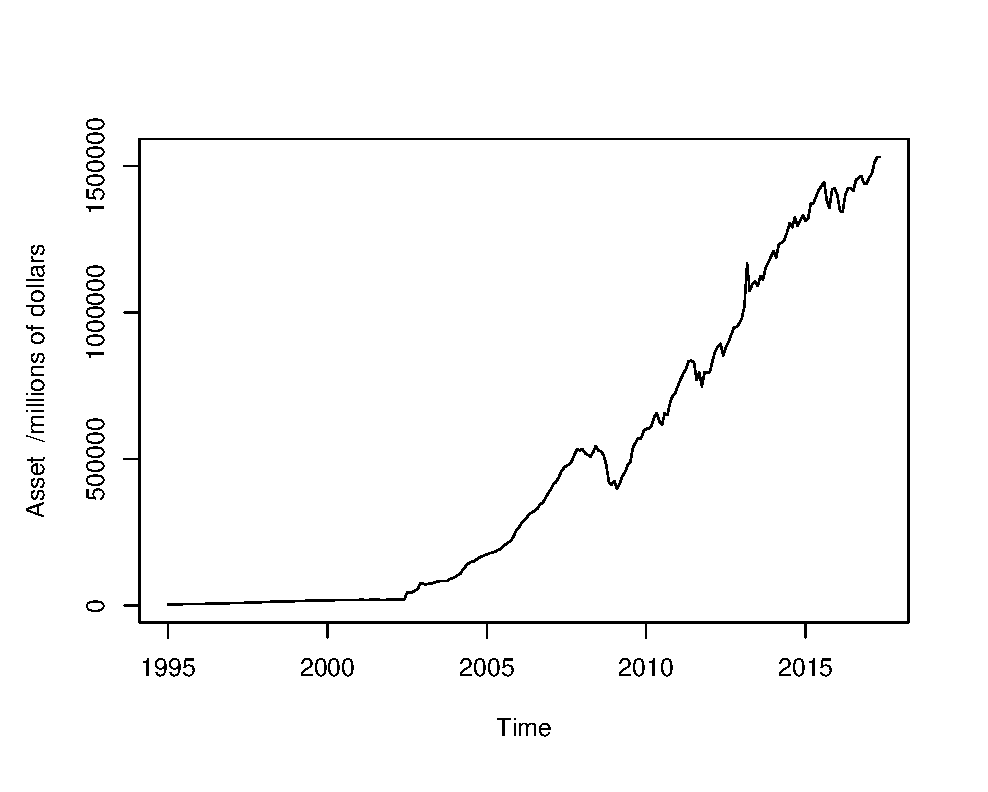
\includegraphics[width=0.5\textwidth]{pic/ast.eps}
	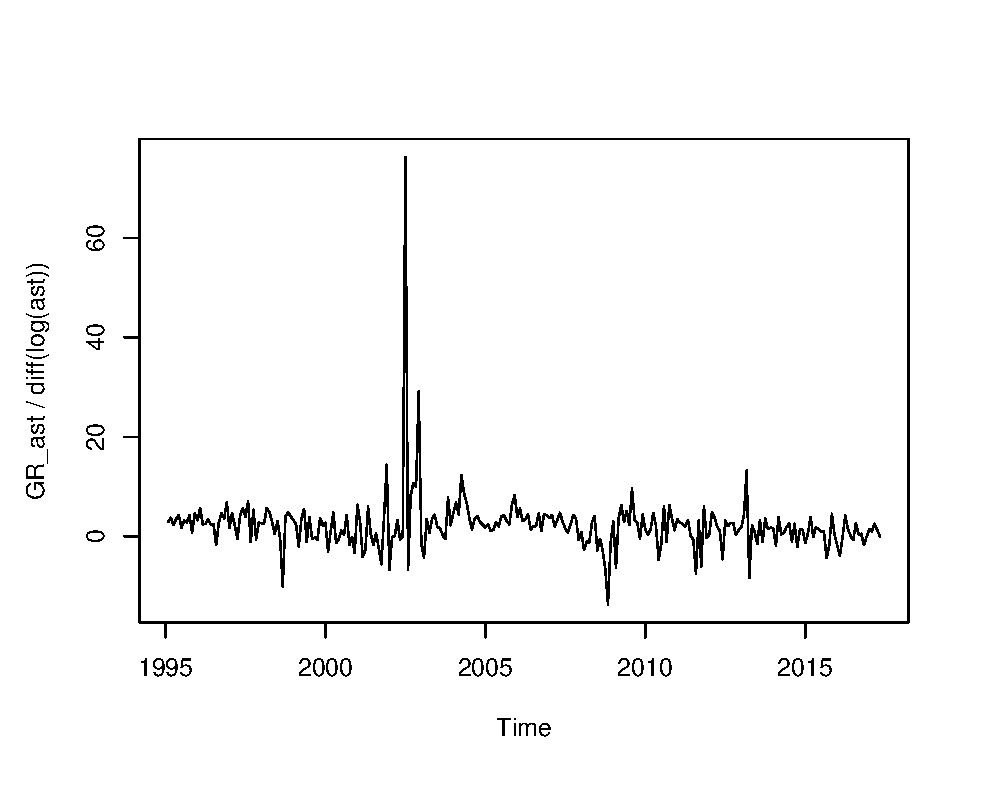
\includegraphics[width=0.5\textwidth]{pic/gr_ast.eps}
\end{figure}

下面对对数差分后的序列进行ARMA建模。绘制$\{GR\_ast_t\}$序列的自相关和偏自相关图像可以发现(图2),此序列的ACF函数在5阶处截尾,PACF函数在5阶处结尾。


\begin{figure}[h!]
\begin{multicols}{2}  
    \begin{minipage}[h]{0.5\textwidth} 
        \centering   
        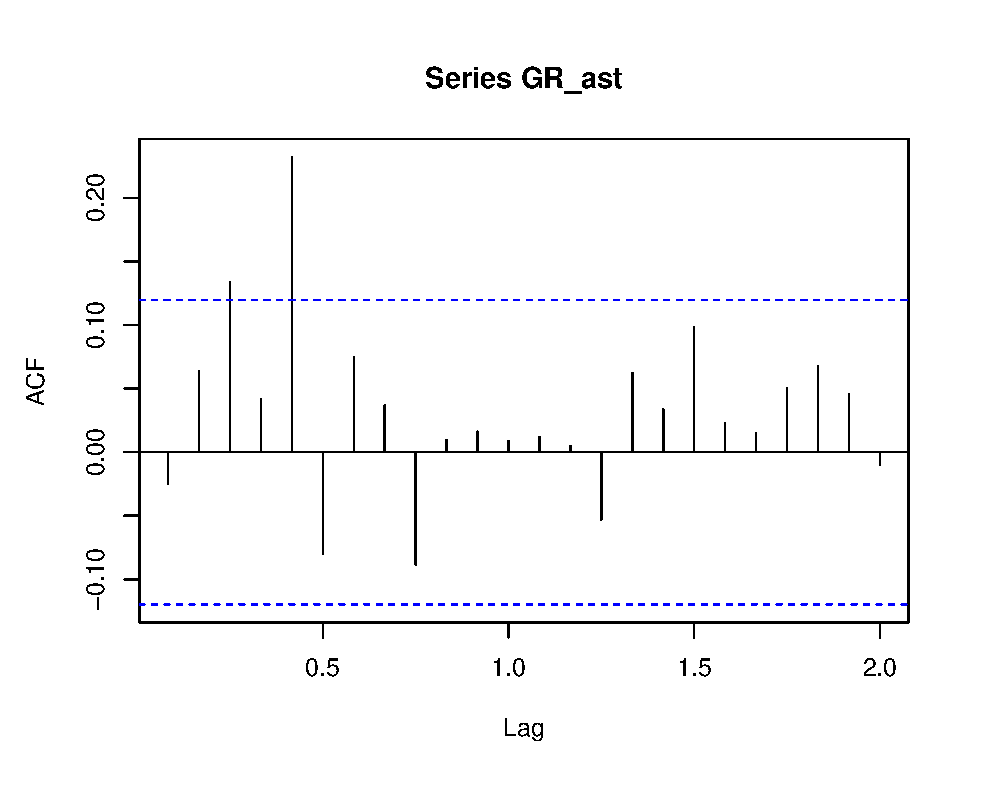
\includegraphics[width=1\textwidth]{pic/acf(gr_ast)}   
        \subcaption{ACF of GR\_ast}   \label{fig:apegrast:a}   
    \end{minipage}
    \begin{minipage}[h]{0.5\textwidth}   
        \centering   
        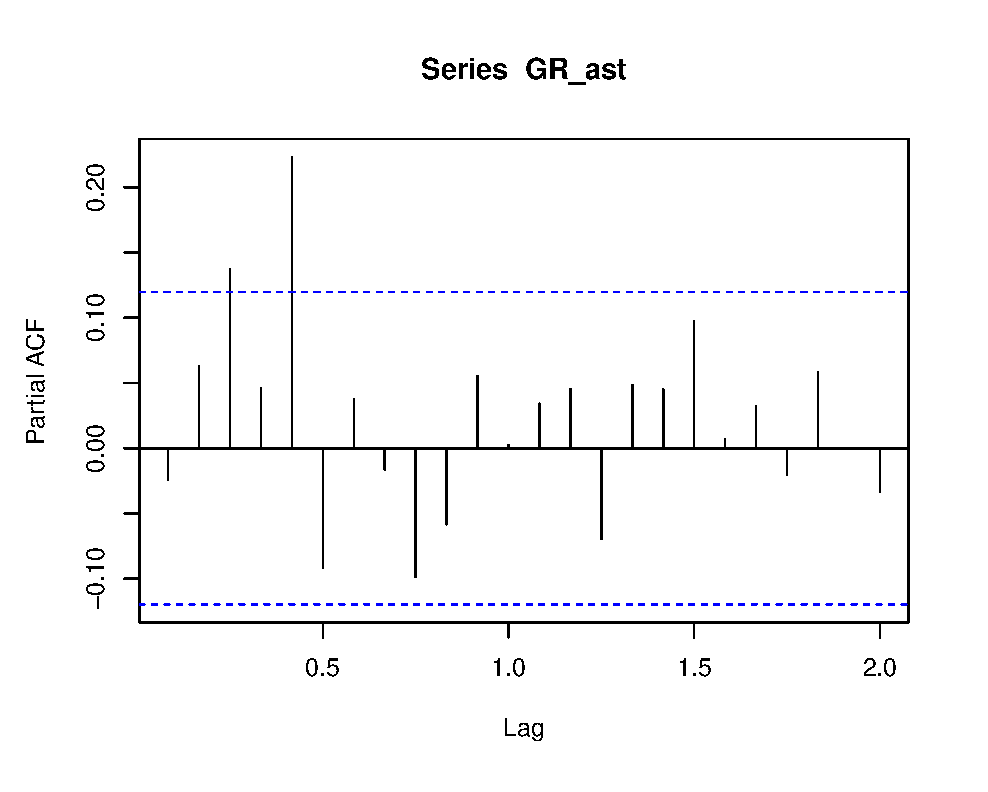
\includegraphics[width=1\textwidth]{pic/pacf(gr_ast)}   
        \subcaption{PACF of GR\_ast}   
        \label{fig:pierce:b}   
    \end{minipage}


    \begin{minipage}[h]{0.5\textwidth} 
        \centering   
        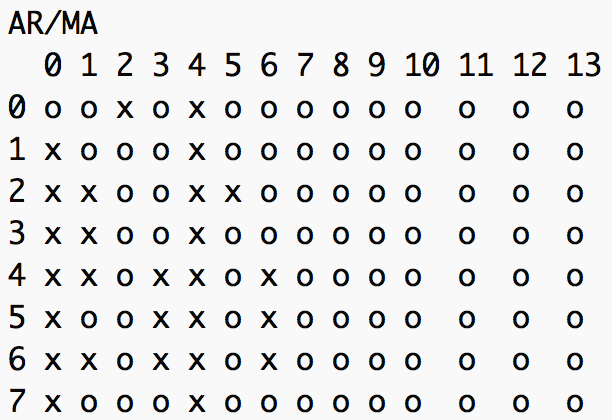
\includegraphics[width=1\textwidth]{pic/eacf(gr_ast)}   
        \subcaption{EACF of GR\_ast}   \label{fig:apegrast:c}   
    \end{minipage}
    \begin{minipage}[h]{0.5\textwidth} 
        \centering   
        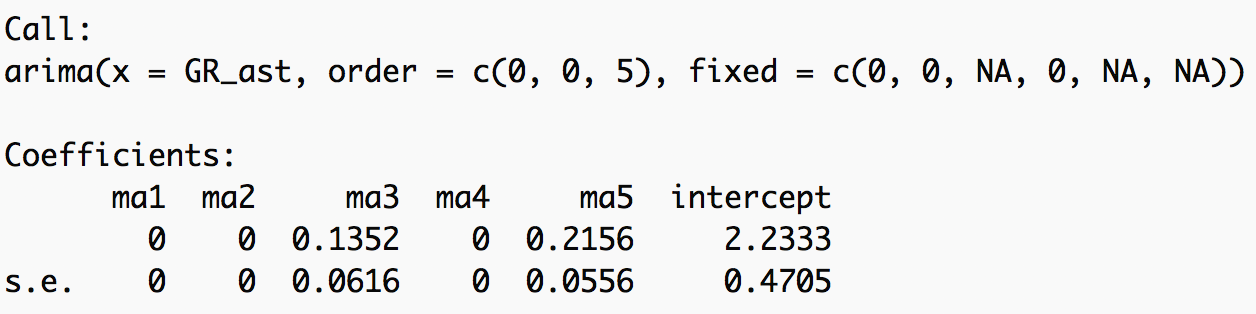
\includegraphics[width=1\textwidth]{pic/ma5}   
        \subcaption{MA Model}   \label{fig:apegrast:d}   
    \end{minipage}    
    \caption{识别MA(q)模型} \label{fig:apegrast}
\end{multicols}
\end{figure}




经过反复尝试,当使用MA(5)对序列进行刻画时,可以得到较好的估计效果。
% MA(5)模型的极大似然估计结果如下:
% MA(5)的极大似然估计结果


\subsection{模型诊断}

对估计的残差$\hat{u_t}$进行Box检验,$p=0.84$,可以接受原假设,满足白噪声要求。同时绘制$\hat{u_t}$的自相关函数,从1阶开始都不显著,也说明$\hat{u_t}$序列不存在自相关。

继续对$\hat{u_t}^2$进行 McLeod.Li检验,判断是否存在ARCH效应。检验结果各阶的p值都接近1,说明不存在ARCH效应。

% 残差估计结果
% 残差平方估计结果
\begin{figure}
\caption{模型诊断}
\begin{multicols}{2}
    \begin{minipage}[h]{0.5\textwidth} 
        \centering   
        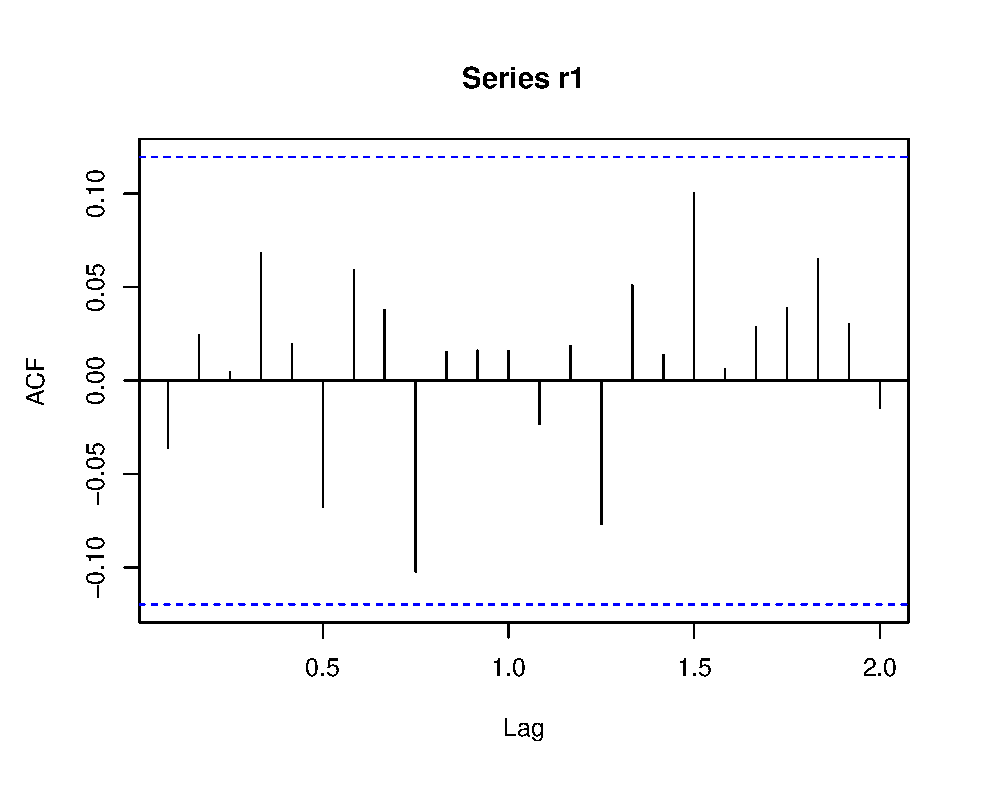
\includegraphics[width=1\textwidth]{pic/acfr1.eps}   
        \subcaption{ACF of residuals}   \label{fig:acfr1}   
    \end{minipage}
    \begin{minipage}[h]{0.5\textwidth}   
        \centering   
        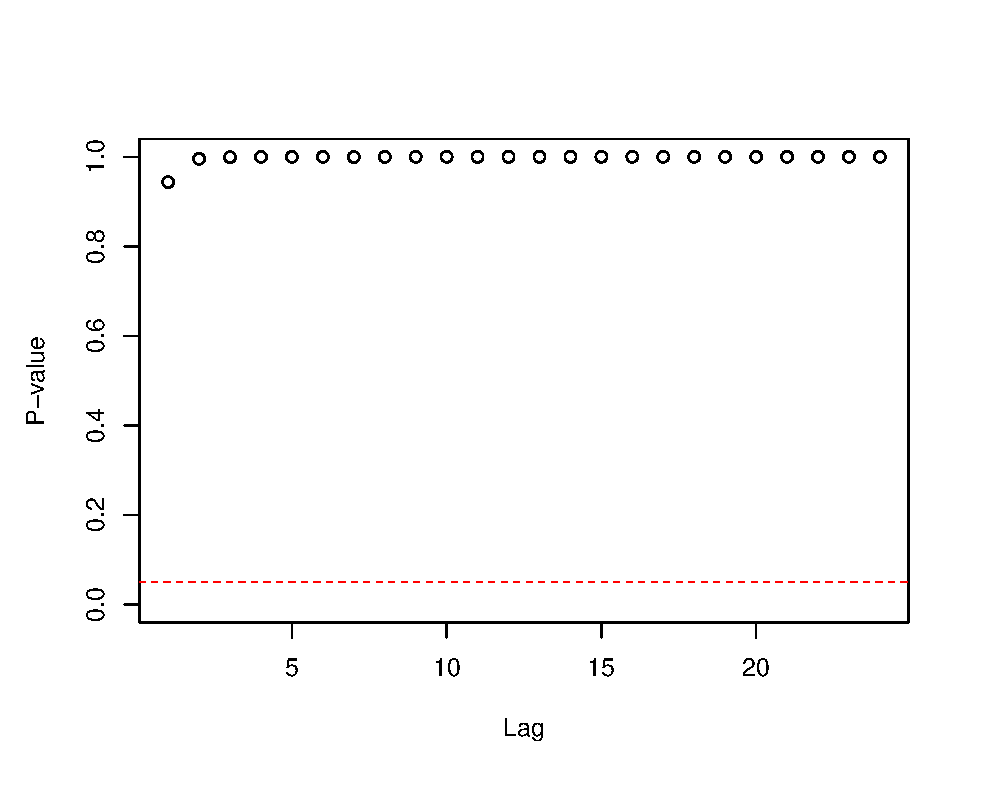
\includegraphics[width=1\textwidth]{pic/mc_gr_ast.eps} 
        \subcaption{McLeod.Li.test of residuals}   
        \label{fig:mcgrast}   
    \end{minipage}
\end{multicols}
\end{figure}

但是,如果绘制出标准化的残差图进行观察,会发现在第90期有一个明显的异常值。很有可能因为这个异常值的出现,使得其他的波动被隐藏,在模型诊断的检验中造成了偏差。通过Bonferroni法则进行检验MA(5)模型,在第90期存在一个强影响点$GR\_ast_{90}$。这进一步确认了我们的猜测(图4)。
% 异常值诊断情况
\begin{figure}
    \caption{异常值诊断}
	\centering
	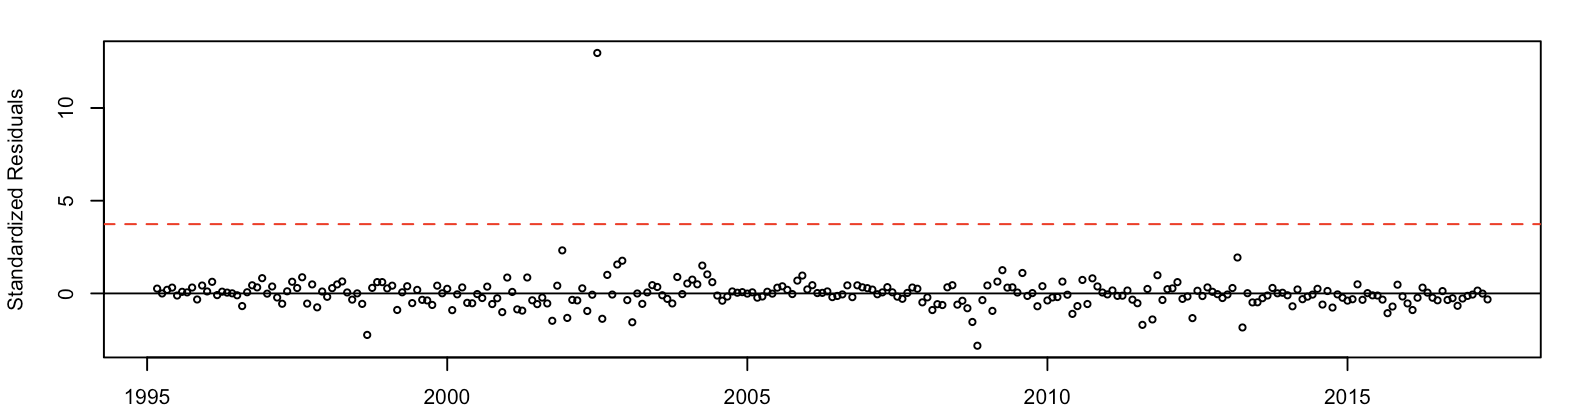
\includegraphics[width=0.8\linewidth]{pic/srgr_ast}
	\subcaption{Standardized Residuals of MA Model for GR\_ast }
	\label{fig:srgrast}
% \end{figure}
% \begin{figure}
	% \centering
	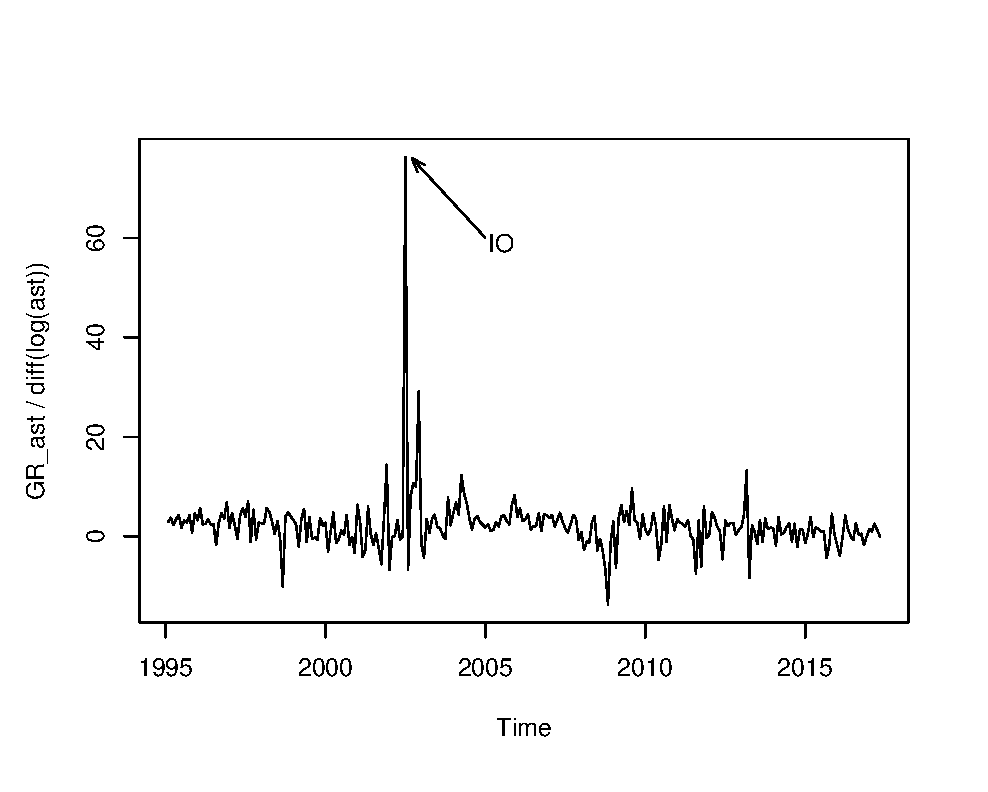
\includegraphics[width=0.5\linewidth]{pic/io}
	\subcaption{Detected outlier}
	\label{fig:io}
\end{figure}


\subsection{异常值处理}
为了削弱第90期的异常值对模型的影响,令
$$GR\_ast_{90} = \frac{1}{3} \cdot (GR\_ast_{89}+GR\_ast_{90}+GR\_ast_{91})$$

\begin{figure}
    \caption{调整后的增长率序列}
	\centering
	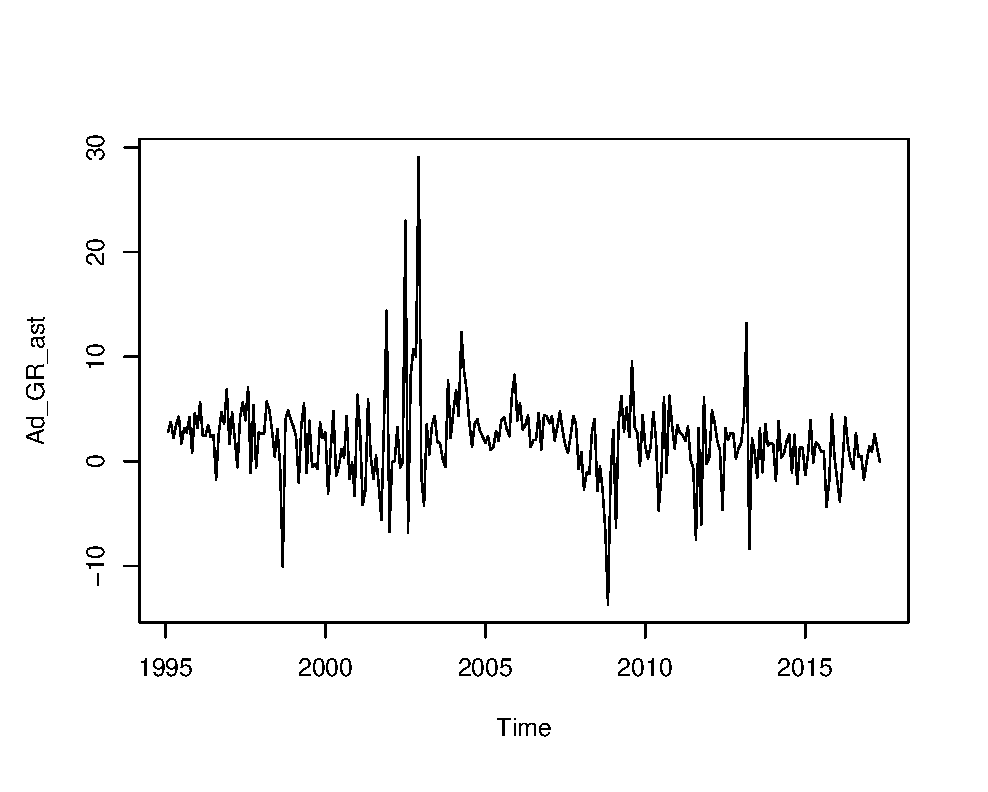
\includegraphics[width=0.5\linewidth]{pic/adgrast}
	\label{fig:adgrast}
\end{figure}

重新对${GR\_ast_t}$序列进行建模估计。
此时对使用极大似然估计得到的残差序列${\hat{u_t}^2}$进行 McLeod.Li检验,检验结果p值很小,拒绝了不存在条件异方差的原假设。即存在GARCH效应(图6)。
% 调整后的存在Garch效应的原模型
\begin{figure}
	\centering
	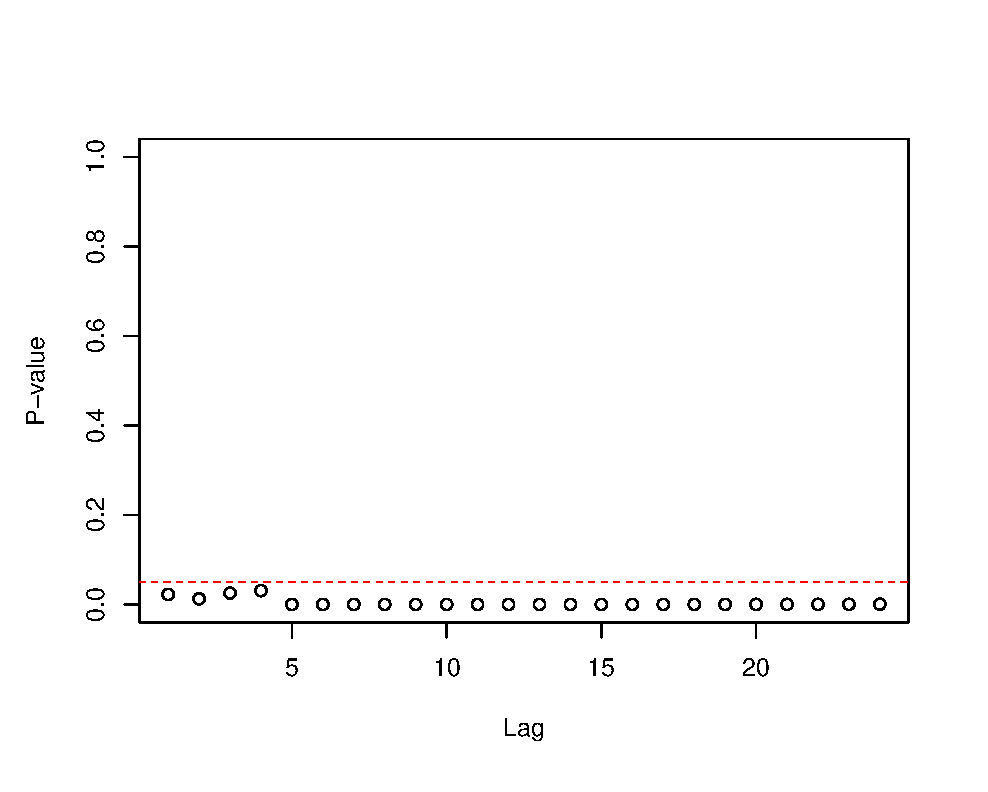
\includegraphics[width=0.5\linewidth]{pic/mcr2}
	\caption{McLeod.Li.test for the residuals of adjusted series}
	\label{fig:mcr2}
\end{figure}

于是使用ARMA(0,5)-GARCH(0,1)对调整后的${GR\_ast_{t}}$进行建模。估计结果如下(图7):

\begin{figure}
	\centering
	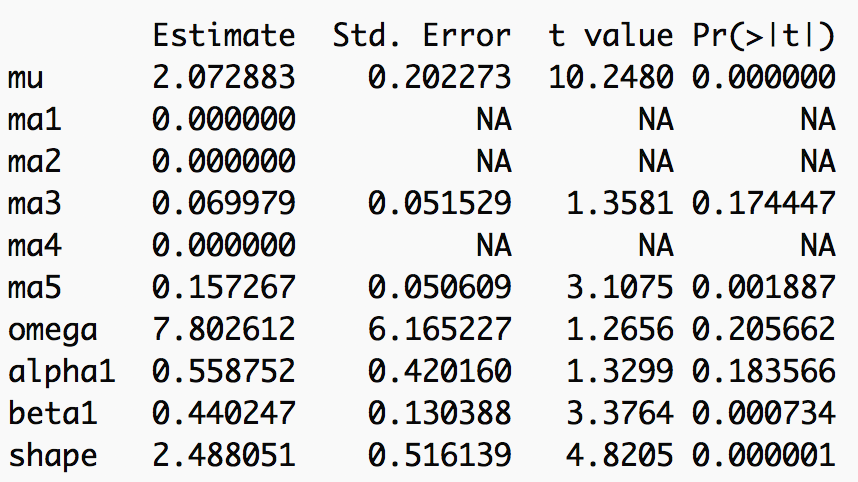
\includegraphics[width=0.7\linewidth]{pic/astgarch}
	\caption{Parameters and t-value,  Distribution	: std }
	\label{fig:astg}
\end{figure}

\section{Cointegration with Retirement Market}
由于美国FOF基金的兴起,主要源于养老金市场的发展。美国雇员逐渐选择将养老金计划由DB转向DC,增大了投资养老金的需求。而FOF基金作为一种收益稳定、风险低的基金,自然受到了这些风险极度厌恶的投资者的青睐。下面,利用彭博数据库中FOF基金资产总量和养老金资产总量的季度数据,对FOF基金市场与养老金市场进行协整分析。在2007-2016十年中,二者的绝对数量和增长率变化趋势如下:

% 两个市场的趋势图像
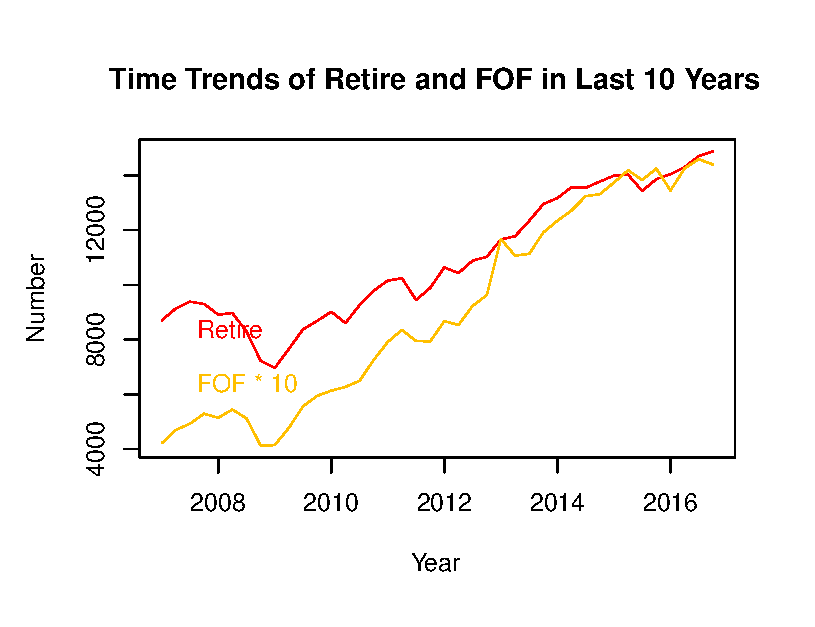
\includegraphics[width=0.4\textwidth]{3-0-1.eps}
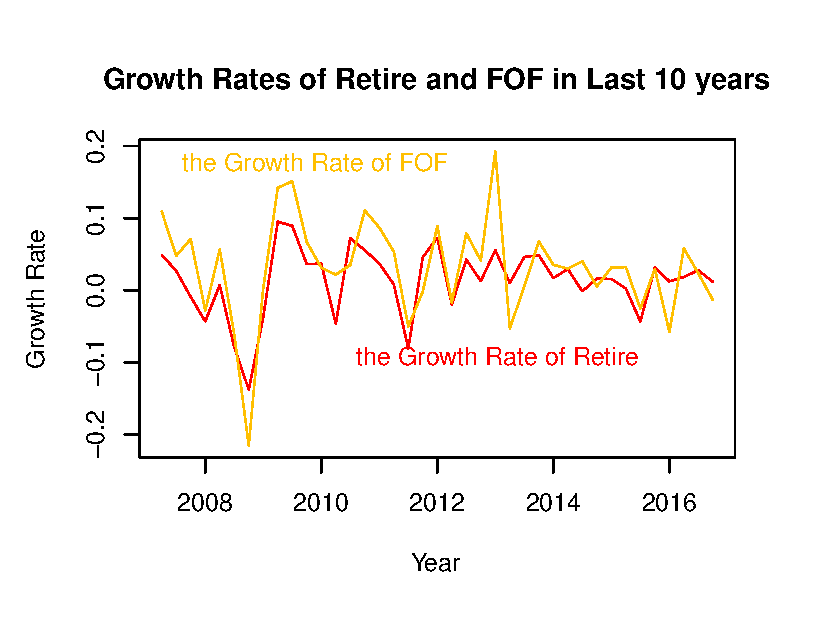
\includegraphics[width=0.4\textwidth]{3-0-2.eps}

% 单位根检验部分
对${FOF_t}$和${Retire_t}$序列分别进行单位根检验。ADF检验和Phillips–Perron的结果接受了原假设(单位根过程),而Kwiatkowski –Phillips–Schmidt–Shin检验结果拒绝了原假设(平稳过程)。因此可以认为${FOF_t}$和${Retire_t}$是非平稳序列。
继续对它们的差分序列${\Delta FOF_t}$和${\Delta Retire_t}$进行单位根检验,得到的结果表明它们是平稳序列。所以,${FOF_t}$和${Retire_t}$分别是2个$I(1)$序列。下面对这两个序列进行协整估计。

% 协整部分
首先,使用最小二乘法估计如下方程:
$$FOF_t = \alpha + \beta \cdot Retire_t + \mu_t$$
得到$\alpha$和$\beta$的估计量$\hat{\alpha}$和$\hat{\beta}$。估计结果如表1:

% OLS回归结果表格
\begin{table}[]
    \centering
    \caption{OLS估计量}
    \label{my-label}
    \begin{tabular}{l | llll}
        Coefficients: &            &            &         &                     \\
                      & Estimate   & Std. Error & t value & Pr(\textgreater|t|) \\  \hline
        (Intercept)   & -7.552e+02 & 5.632e+01  & -13.41  & 5.51e-16 ***        \\
        Retire        & 1.524e-01  & 5.042e-03  & 30.22   & \textless 2e-16 ***
    \end{tabular}
\end{table}


对残差估计序列${\hat{u_t}}$进行单位根检验,${\hat{u_t}}$在ADF检验和PP检验中拒绝了原假设,在KPSS检验中接受了原假设。
因此可以认为${FOF_t}$和${Retire_t}$两个$I(1)$过程得到了平稳的$I(0)$
过程。即两个序列之间存在着长期的均衡关系(协整关系)。协整向量为$(1, -0.15)$

% 残差具有平稳性
\begin{table}[]
    \centering
    \caption{OLS估计残差的单位根检验}
    \label{my-label}
    \begin{tabular}{l | llll}
        Tests        & ADF-Test       & KPSS-Test      & PP-Test               \\  \hline
        Statistics   & -3.1799 (<1pct & 0.2674(<10pct) & -10.0379 (<Z-tau)  
    \end{tabular}
\end{table}

% Error Correction Model
记$y_t = FOF_t$,$x_t = Retire_t$,建立误差修正模型。由于使用的是季度数据,所以加入$\Delta y_t$的1-4阶滞后项。
$$\Delta y_t = \alpha_1 \cdot \Delta y_{t-1} + \alpha_2  \cdot \Delta  y_{t-2} + \alpha_3 \cdot \Delta  y_{t-3} + \alpha_4 \cdot \Delta  y_{t-4} + \beta_0 \cdot \Delta  x_t+\beta_1 \cdot \Delta  x_{t-1} + +\gamma \cdot ( y_{t-1}-kx_{t-1}) + \epsilon_t$$


估计结果表3:
\begin{table}[]
    \centering
    \caption{误差修正模型估计结果}
    \label{my-label}
    \begin{tabular}{l | llll}
        Coefficients: &          &            &         &                     \\
                      & Estimate & Std. Error & t value & Pr(\textgreater|t|) \\  \hline
        (Intercept)   & 22.13335 & 11.14436   & 1.986   & 0.0573              \\
        L(y, 1)       & -0.46108 & 0.19994    & -2.306  & 0.029 *             \\
        L(y, 2)       & -0.01601 & 0.12908    & -0.124  & 0.9022              \\
        L(y, 3)       & -0.03563 & 0.12999    & -0.274  & 0.7861              \\
        L(y, 4)       & -0.02875 & 0.13862    & -0.207  & 0.8373              \\
        L(x, 1)       & 0.05842  & 0.02549    & 2.292   & 0.03 *              \\
        L(x, 0)       & 0.09517  & 0.01852    & 5.138   & 0.000021 ***        \\
        L(r, 1)       & -0.38373 & 0.16855    & -2.277  & 0.0309 *           
    \end{tabular}
\end{table}


误差修正项的系数在10\%的程度显著。协整向量为$(1, -0.15)$。


\section{Conclusion}
    \begin{enumerate}
        \item 在过去的20年中,$FOF$资产总量的增长率满足$ARMA(0,5) \sim GARCH(1,1)$模型。
        \item FOF基金市场和养老金市场之前存在协整关系。FOF资产总量维持在养老金市场总量的15\%水平,可以实现长期稳定关系。
    \end{enumerate}
\end{document}
